%%%%%%%%%%%%%%%%%%%%%%%%%%%%%%%%%%%%%%%%%
\section{Agenda}
\begin{frame}{Agenda}
\begin{itemize}
\item Problem introduktion
\item Eksisterende modeller
\item Parameter bestemmelse
\item Databehandling
\item Parameternes betydning
\item Foreslået PL model
\item Model sammenligning
\item z parameteren
\item Konklusion
\end{itemize}
\end{frame}
%%%%%%%%%%%%%%%%%%%%%%%%%%%%%%%%%%%%%%%%%
\section{Problem introduktion}
\begin{frame}{Problem introduktion}
\begin{minipage}{0.5\textwidth}

\begin{itemize}
\item Lavstående antenner.
\item Kommunikation mellem nodes og basestationer.
\item Ikke idealle forhold
\item Jorden og andre objekters påvirkning kan ikke længere negleres.
\end{itemize}

\end{minipage}
\begin{minipage}{0.45\textwidth}

\begin{figure}[!htbp]
 \centering
  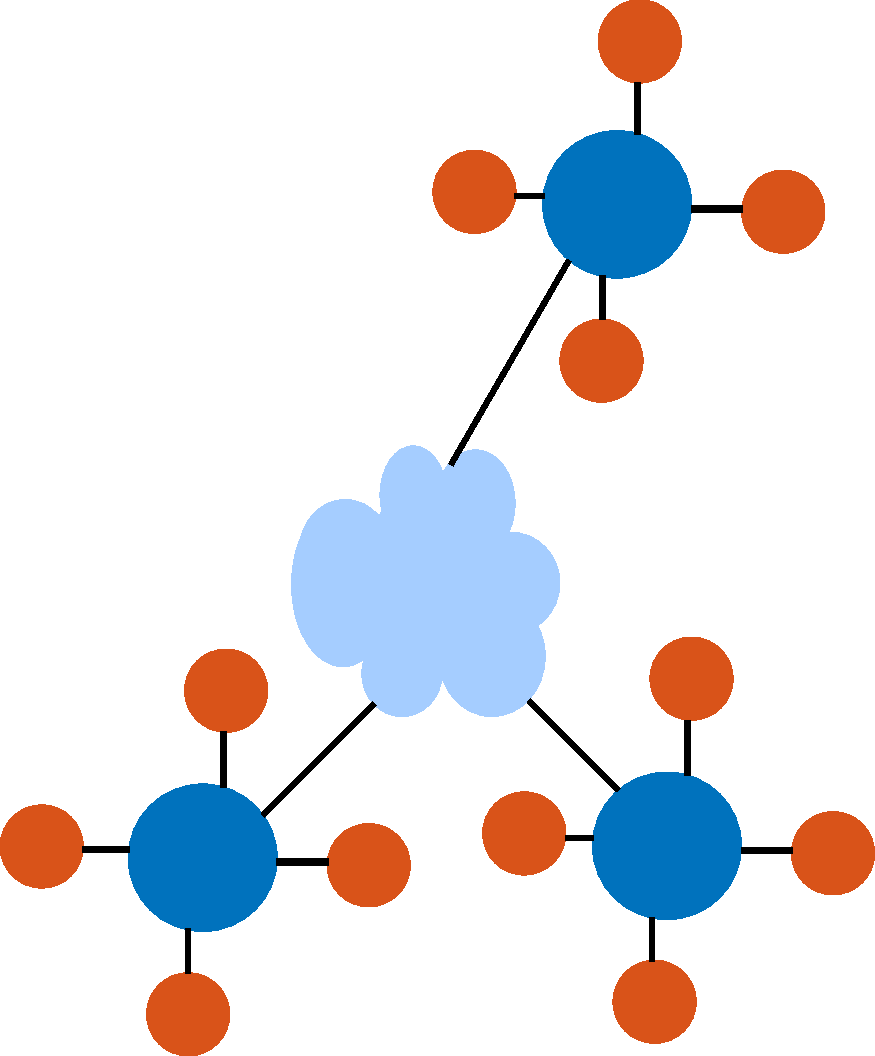
\includegraphics[width = \columnwidth]{figures/wsn_ill.pdf}
  \end{figure}

\end{minipage}
\end{frame}

%%%% Signaler
\begin{frame}{Problem introduktion}
\begin{minipage}{0.5\textwidth}

\begin{itemize}
\item Projekt begrænsninger
\begin{itemize}
\item Line of sight (LOS)
\item Kun refleksion fra fladt underlag
\item Ingen forstyrrende elemeter
\item Konstant signal styrke
\end{itemize}
\end{itemize}

\end{minipage}
\begin{minipage}{0.45\textwidth}

\begin{figure}[!htbp]
 \centering
  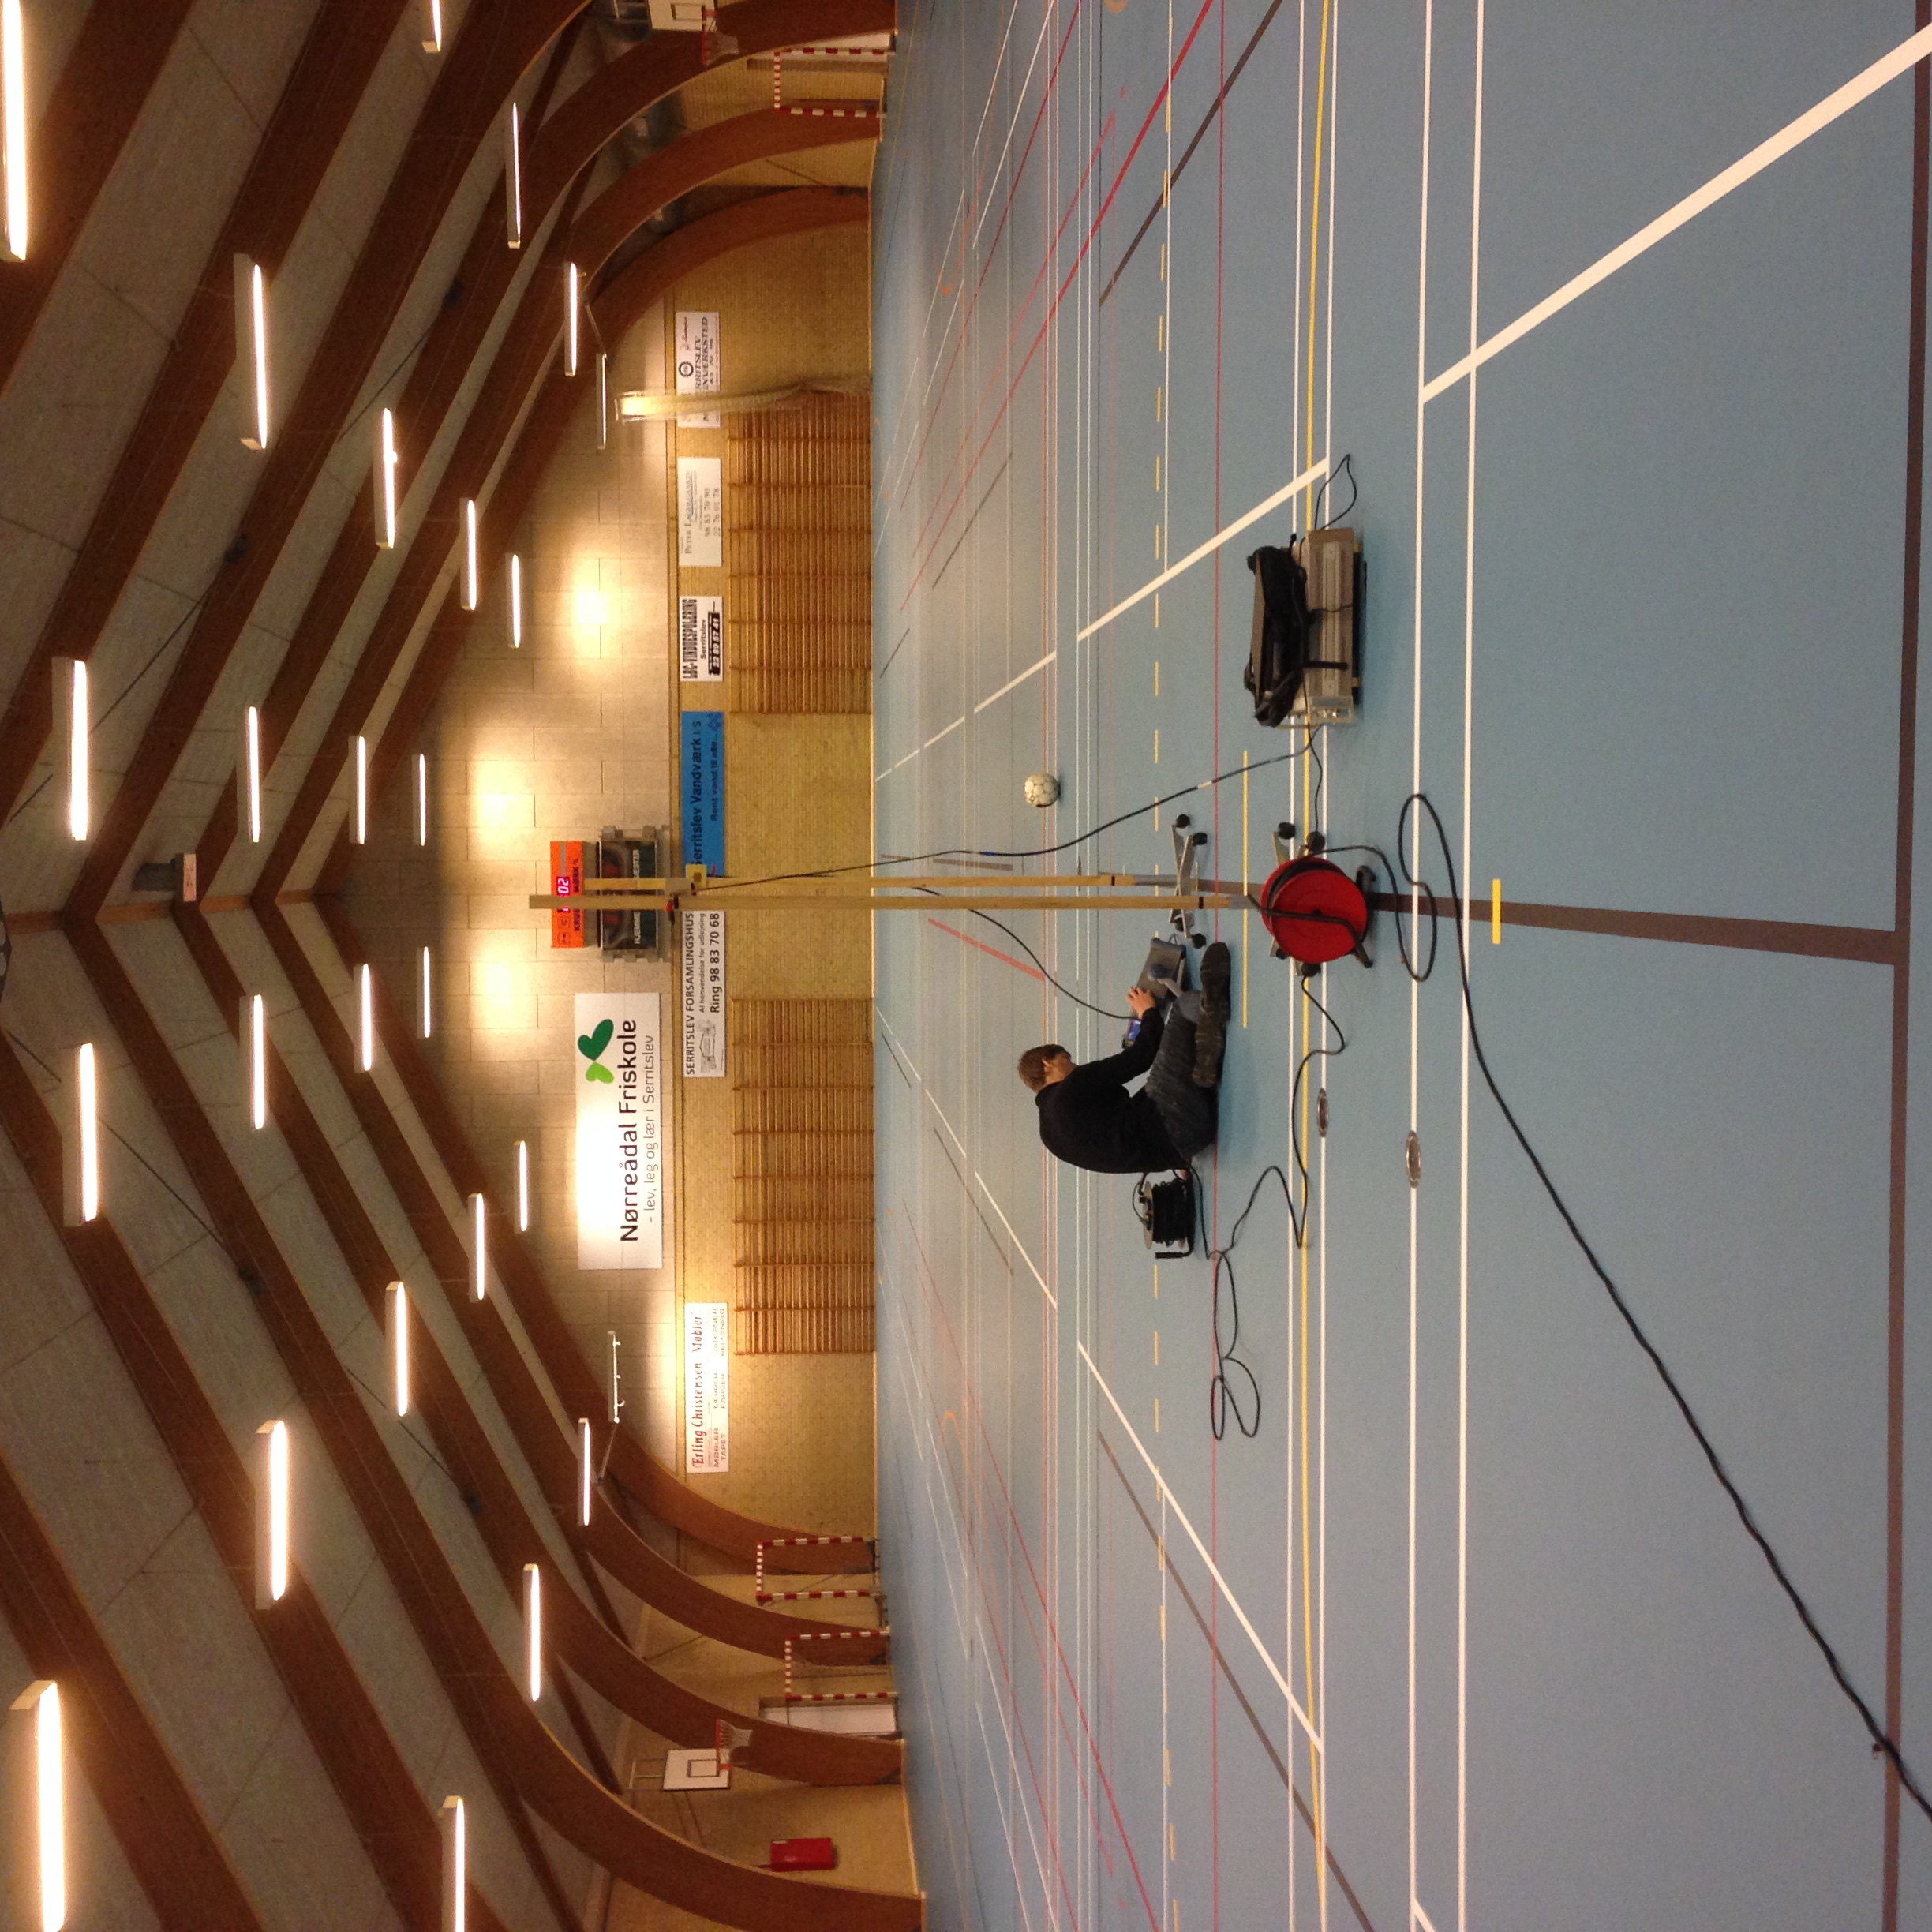
\includegraphics[width = \columnwidth, angle = -90]{figures/Hal.jpg}
  \end{figure}

\end{minipage}
\end{frame} 
 
%%%%%%%%%%%%%%%%%%%%%%%%%%%%%%%%%%%%%%%
\begin{frame}{Exiterende modeller}
\begin{minipage}{.45\textwidth}
\raggedright\textcolor{thomaspurple}{\textbf{Ground wave PL (GWPL)}:}
\begin{itemize}
\item Alle bølger
\item Alle højder
\item Flade konstanter nødvendige
\end{itemize} 

\vspace{1em}
\textcolor{black}{\textbf{Krav:}}
\begin{itemize}
\item LOS og ingen forstyrrende elementer
\item Flad overflade
\end{itemize}

\end{minipage}
\begin{minipage}{0.5\textwidth}
\begin{figure}[!htbp]
 \centering
  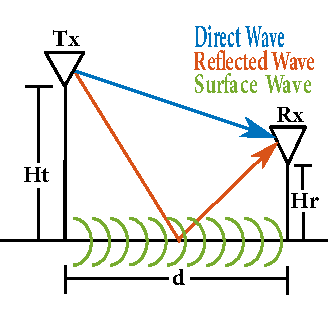
\includegraphics[width = \columnwidth]{figures/poster_cropped_1.pdf}
  \end{figure}
\end{minipage}

\vspace{1em}
\begin{equation}
L_p=\left(\frac{4 \pi d}{\lambda}\right)^2 \cdot \Big|\underbrace{1}_{\begin{subarray}{c}Direct\\wave\end{subarray}}+\underbrace{R\text{e}^{j\Delta}}_{\begin{subarray}{c}Reflected\\wave\end{subarray}}+\underbrace{(1-R)A\text{e}^{j\Delta}}_{\begin{subarray}{c}Surface\\wave\end{subarray}}\Big|^{-2} 
\label{ground_wave}
\end{equation}
\end{frame}


\section{Exiterende modeller}
\begin{frame}{Exiterende modeller}
\begin{minipage}{.45\textwidth}
\raggedright\textcolor{thomasblue}{\textbf{Friss free space PL (FSPL)}:}
\begin{itemize}
\item LOS og ingen forstyrrende elementer
\item Kun den direkte bølge
\item Høje højder
\end{itemize} 

\vspace{1em}
\textcolor{black}{\textbf{Krav:}}
\begin{itemize}
\item Ingen reklsioner eller ekstra signaler
\item LOS
\item $d >> \lambda$
\end{itemize}
\end{minipage}
\begin{minipage}{0.5\textwidth}

\begin{figure}[!htbp]
 \centering
  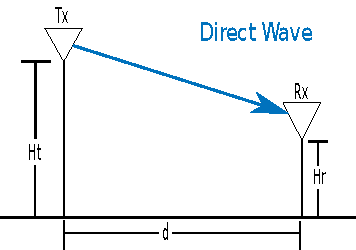
\includegraphics[width = \columnwidth]{figures/friss_illu.pdf}
  \end{figure}
\end{minipage}

\vspace{1em}
\begin{equation*}
L_p=\left(\frac{4 \pi d}{\lambda}\right)^2
\end{equation*}
\end{frame}


\begin{frame}{Exiterende modeller}
\begin{minipage}{.45\textwidth}
\raggedright\textcolor{thomasred}{\textbf{Approximated two-ray}}\\
\raggedright\textcolor{thomasred}{\textbf{ground-reflection PL (ATRPL)}:}
\begin{itemize}
\item Direkte og reflekteret bølger
\item Mellem højder til lave højder
\end{itemize} 

\vspace{1em}
\textcolor{black}{\textbf{Krav:}}
\begin{itemize}
\item LOS og ingen forstyrrende elementer
\item Flad overflade
\item $d > \frac{4\pi \cdot h_t h_r }{\lambda}$
\end{itemize}

\end{minipage}
\begin{minipage}{0.5\textwidth}
\begin{figure}[!htbp]
 \centering
  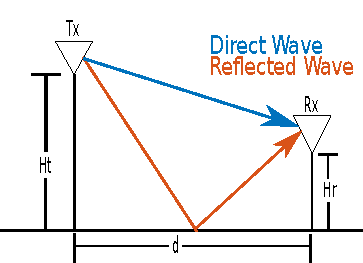
\includegraphics[width = \columnwidth]{figures/two_ray_illu.pdf}
  \end{figure}
\end{minipage}

\vspace{1em}
\begin{equation*}
L_{p} = \left(\frac{d^2}{h_t h_r}\right)^2
\label{two_ray_model}
\end{equation*}
\end{frame}


\begin{frame}{Exiterende modeller}
\begin{minipage}{.45\textwidth}
\raggedright\textcolor{thomasgreen}{\textbf{Norton surface wave PL (NSPL)}:}
\begin{itemize}
\item Overflade bølgen
\item Lave højder
\item Flade konstanter nødvendige
\end{itemize}

\vspace{1em}
\textcolor{black}{\textbf{Krav:}}
\begin{itemize}
\item LOS og ingen forstyrrende elementer
\item Flad overflade
\item $h_t,h_r > \lambda$
\end{itemize}

\end{minipage}%
\begin{minipage}{0.5\textwidth}
\begin{figure}[!htbp]
 \centering
  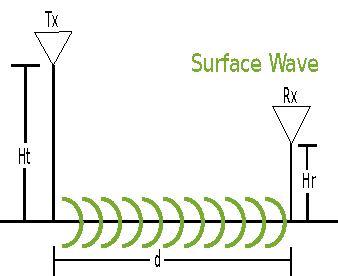
\includegraphics[width = \columnwidth]{figures/surf_illu.pdf}
  \end{figure}
\end{minipage}

\vspace{1em}
\begin{equation}
L_p=\left({d} \cdot \left|\frac{\lambda}{2\pi z}\right|^{-1}\right)^4
\label{surface_wave}
\end{equation}
\end{frame}





%%%%%%%%%%%%%%%%%%%%%%%%%%%%%%%%%%%%
\section{Parameter bestemmelse}
\begin{frame}{Parameter bestemmelse}
\begin{figure}[!htbp]
	\centering
	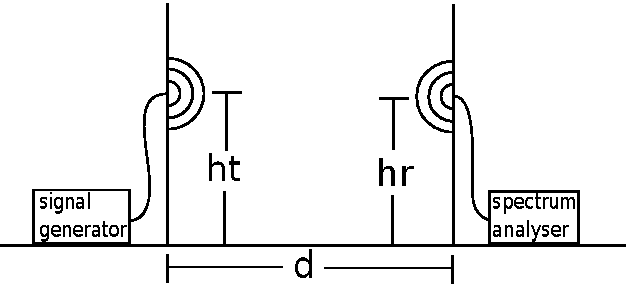
\includegraphics[width = 0.8\columnwidth]{figures/setup.pdf}
\end{figure}
\begin{minipage}{0.15\textwidth}
 \textcolor{white}{.}  
\end{minipage}%
\begin{minipage}{0.8\textwidth}
\begin{itemize}
\item Frekvenser
\item Antenne par
\item Polarisering
\item Lokationer
\item Rx/Tx højder
\item Afstande
\end{itemize}
\end{minipage}
\end{frame}

\begin{frame}{Parameter bestemmelse}
\begin{figure}[!htbp]
	\centering
	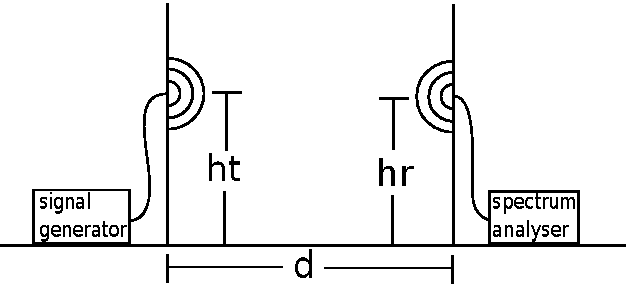
\includegraphics[width = 0.8\columnwidth]{figures/setup.pdf}
\end{figure}
\begin{minipage}{0.15\textwidth}
 \textcolor{white}{.}  
\end{minipage}%
\begin{minipage}{0.8\textwidth}
\begin{itemize}
\item Flere målinger per punkt (10 stk.) \pause
\item Antal af de forskellige parameter
\begin{itemize}
\item Hvis der er 2 af hver parameter, vil det kræve 1280 målinger
\item Hvis der er 5 af hver parameter, vil det kræve 781250 \pause
\end{itemize}
\item Noget skal der gøres ved dette!
\end{itemize}
\end{minipage}
\end{frame}

\begin{frame}{Parameter bestemmelse}
\begin{figure}[!htbp]
	\centering
	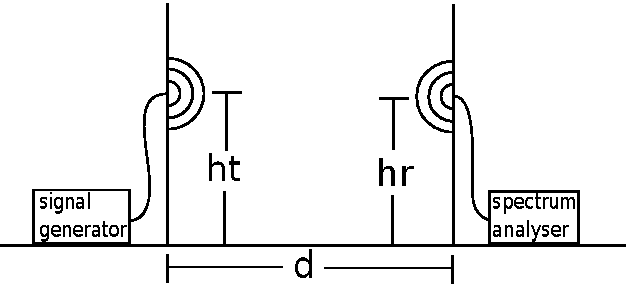
\includegraphics[width = 0.8\columnwidth]{figures/setup.pdf}
\end{figure}
\begin{minipage}{0.15\textwidth}
 \textcolor{white}{.}  
\end{minipage}%
\begin{minipage}{0.8\textwidth}
\begin{itemize}
\item Vigtige parameter:
\begin{itemize}
\item Højder og afstande
\end{itemize}
\item Mindre vigtige parameter:
\begin{itemize}
\item Antenner, polarisering, frekvens og lokation
\end{itemize}
\end{itemize}
\end{minipage}
\end{frame}

\begin{frame}{Parameter bestemmelse}
\begin{figure}[!htbp]
	\centering
	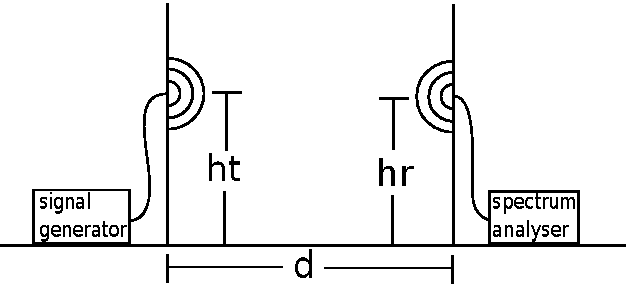
\includegraphics[width = 0.8\columnwidth]{figures/setup.pdf}
\end{figure}
\begin{minipage}{0.15\textwidth}
 \textcolor{white}{.}  
\end{minipage}%
\begin{minipage}{0.8\textwidth}
\begin{itemize}
	\item Antenne par
	\begin{itemize}
		\item Kræver to antenner, en til at sende og en til at modtage
		\item Simple konstrution, samt simpelt udstrålings mønster
		\item Monopol og patch antenner
	\end{itemize}
	\item Frekvens
	\begin{itemize}
		\item Kræver helt nye antenner per frekvens
	\end{itemize}
\end{itemize}
\end{minipage}
\end{frame}

\begin{frame}{Parameter bestemmelse}
\begin{minipage}{0.45\textwidth}
\begin{figure}[!htbp]
	\centering
	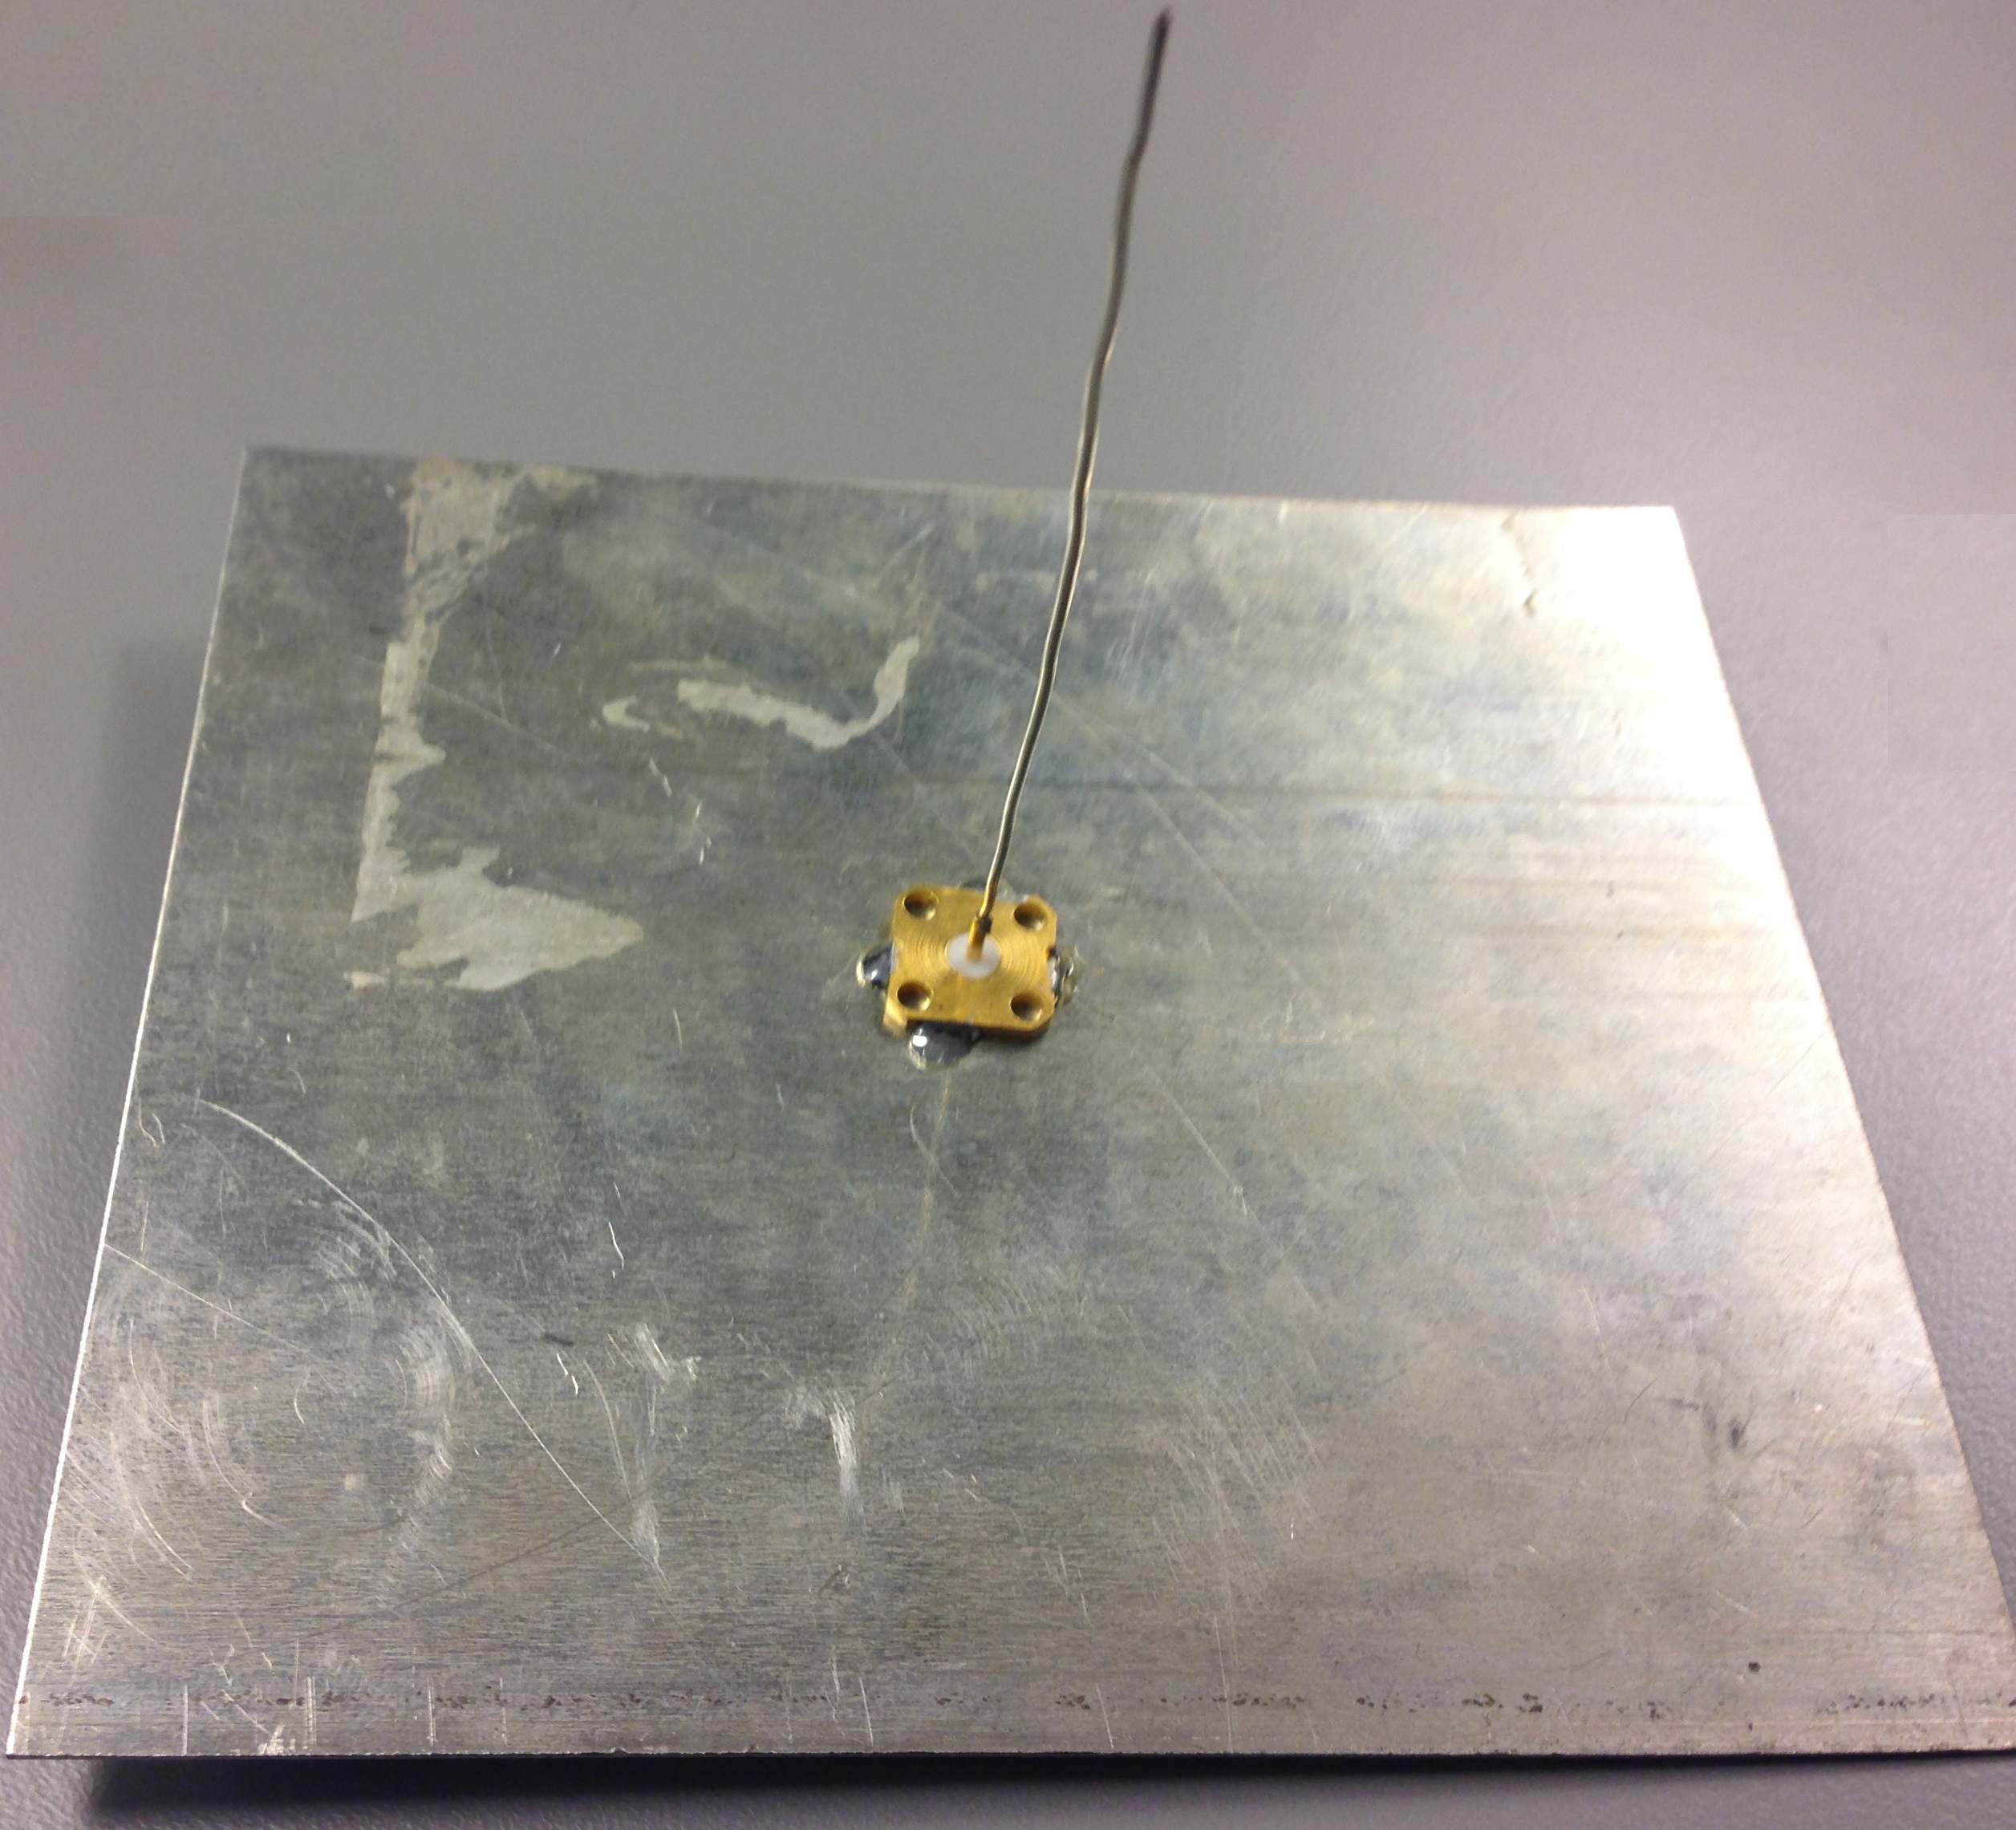
\includegraphics[width = 0.87\columnwidth]{figures/MonoAnt.jpg}\\
	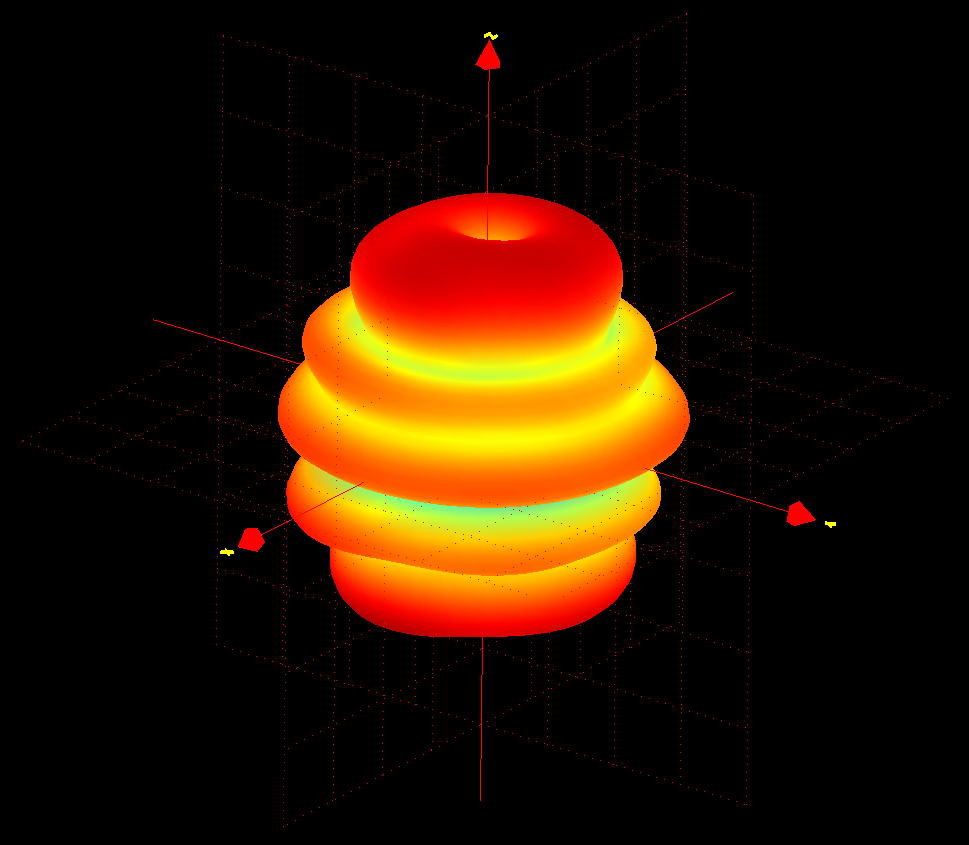
\includegraphics[width = 0.87\columnwidth]{figures/MonoStor2500.png}
\end{figure}
\end{minipage}%
\begin{minipage}{0.1\textwidth}
\textcolor{white}{.} 
\end{minipage}%
\begin{minipage}{0.45\textwidth}
\begin{figure}[!htbp]
	\centering
	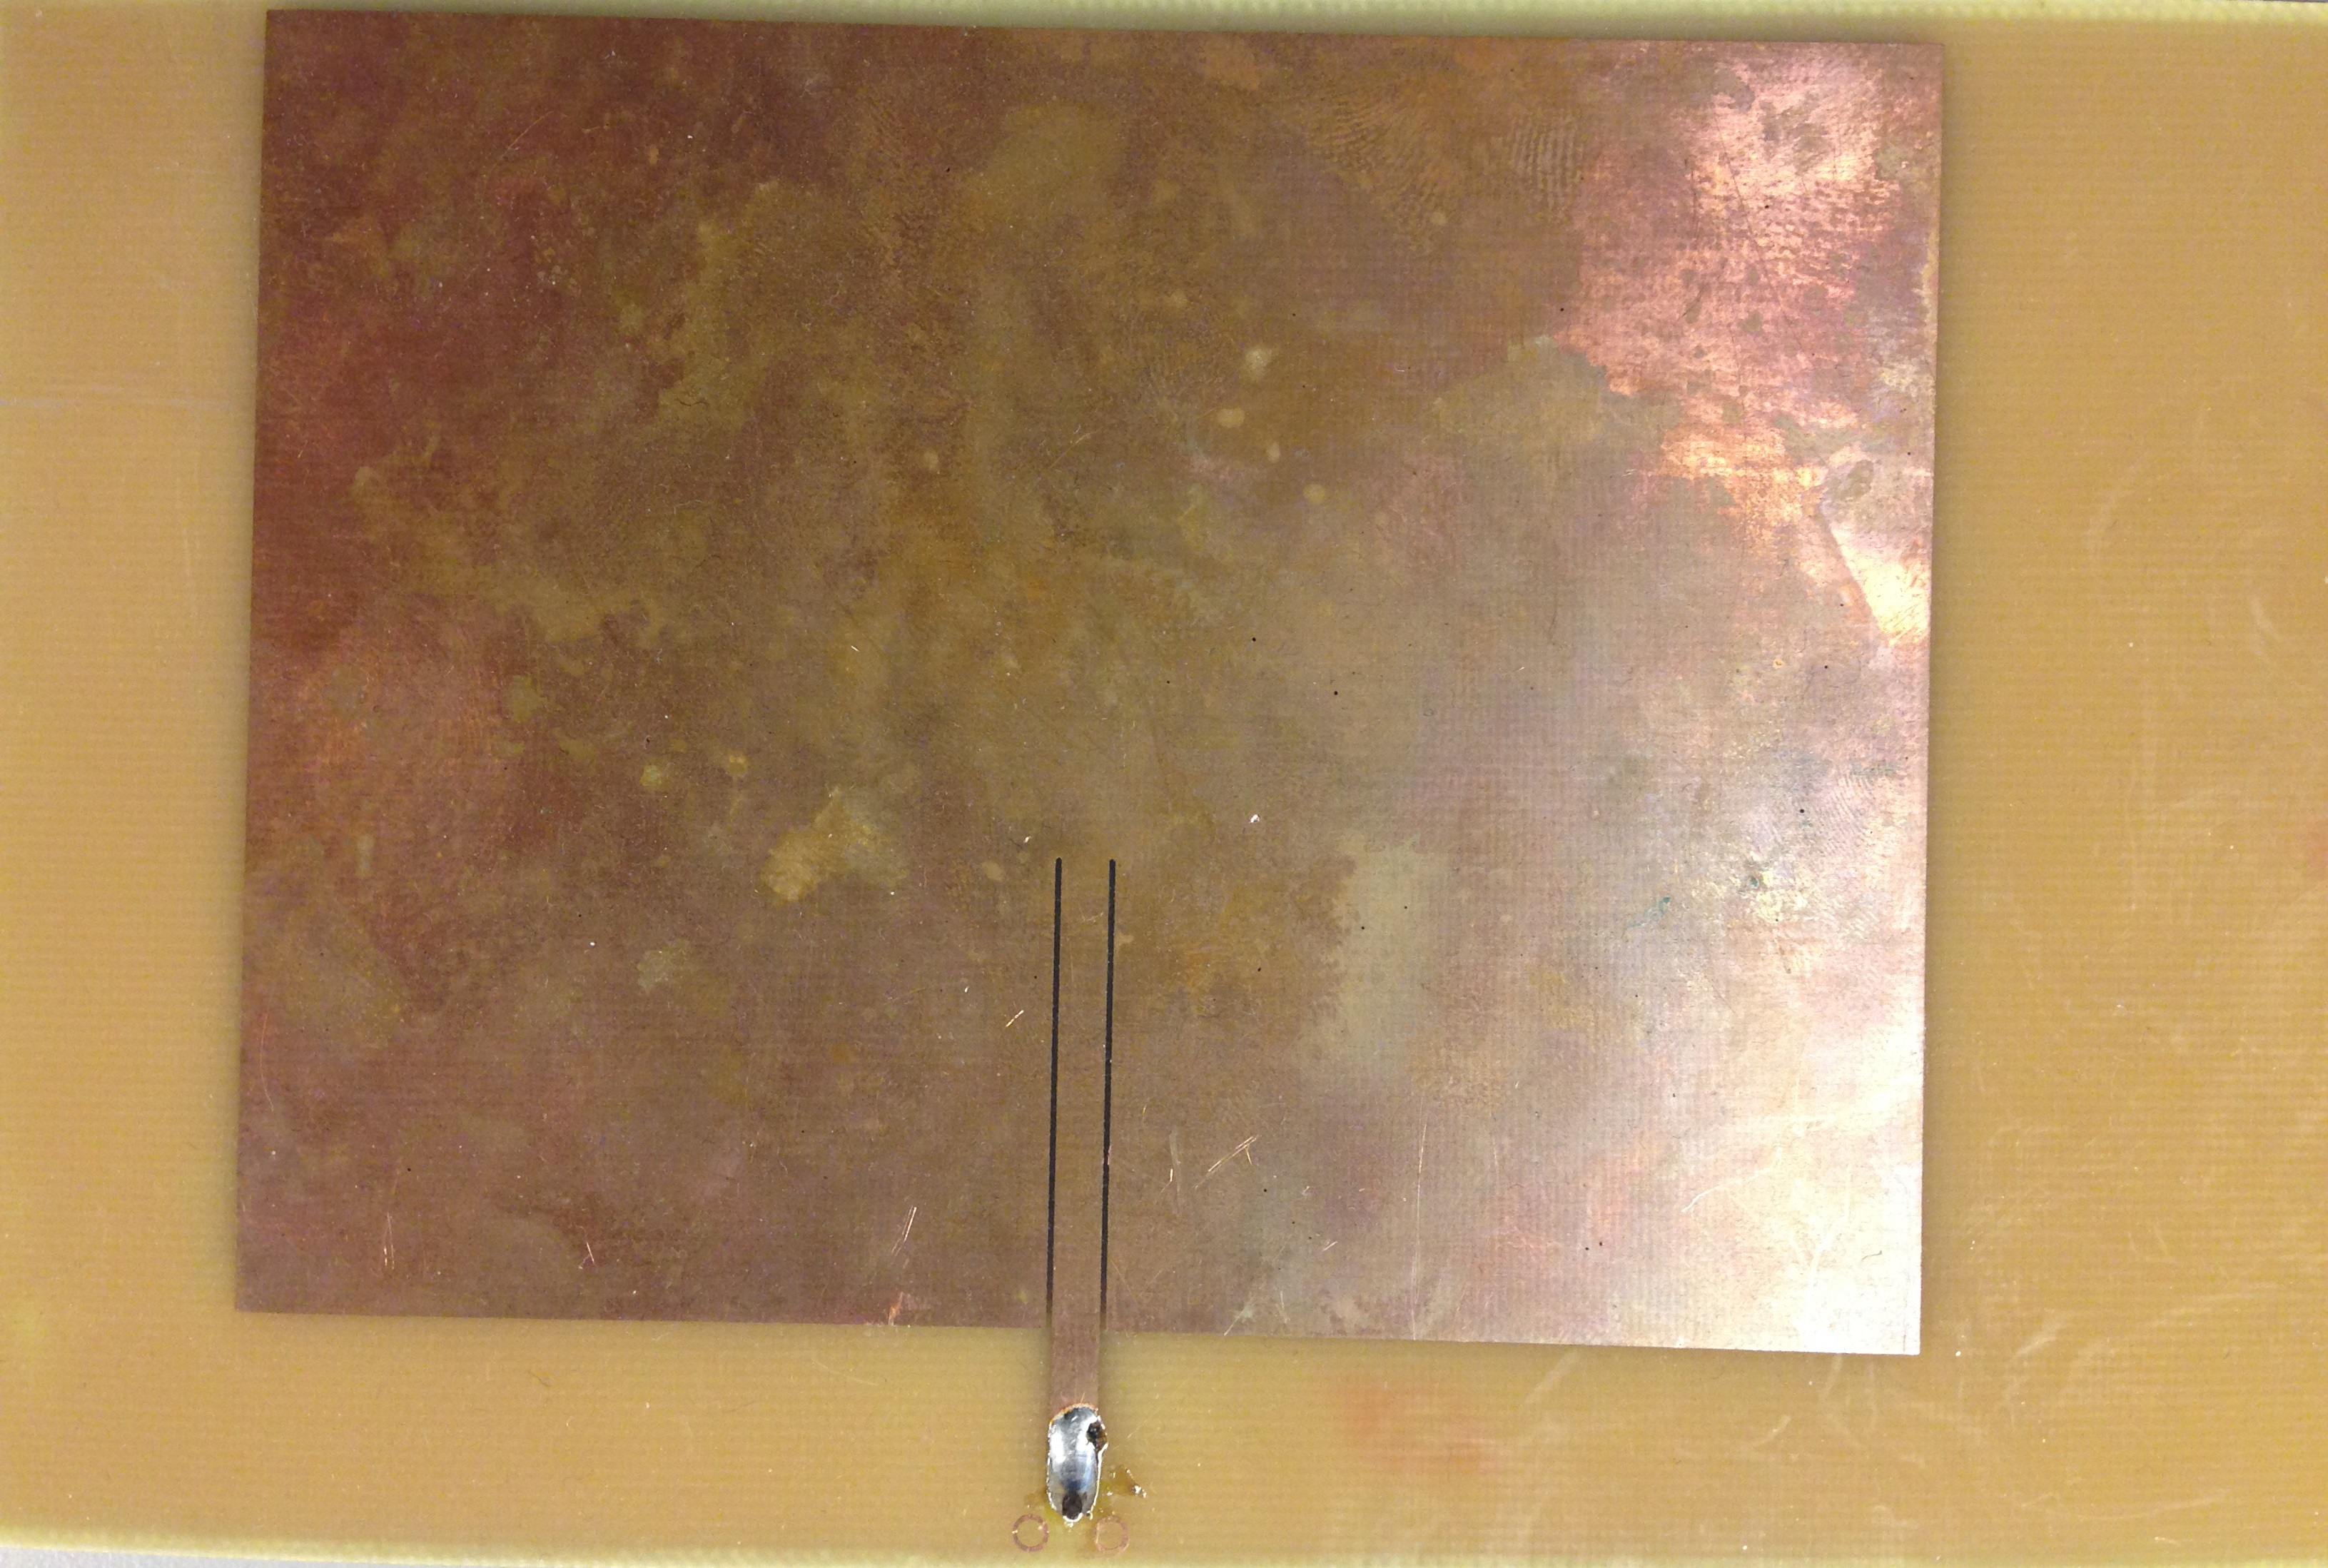
\includegraphics[width = \columnwidth]{figures/PatchAnt.jpg}\\
	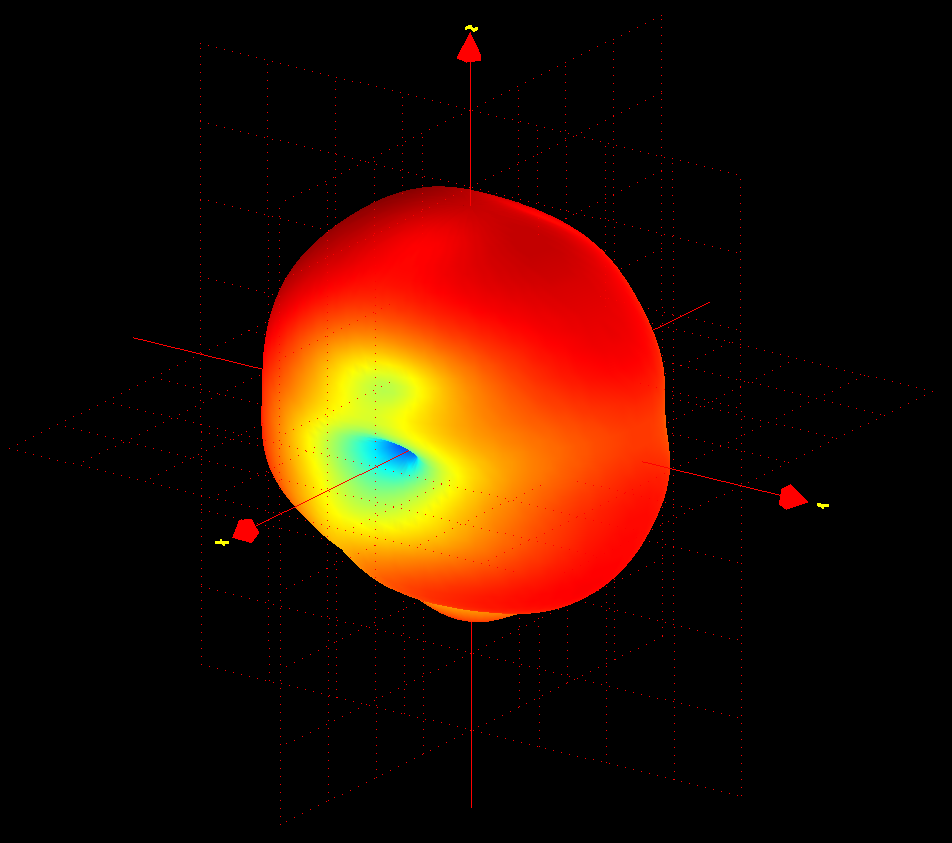
\includegraphics[width = \columnwidth]{figures/PatchNy858.png}
\end{figure}
\end{minipage}
\end{frame}

\begin{frame}{Parameter bestemmelse}
\begin{figure}[!htbp]
	\centering
	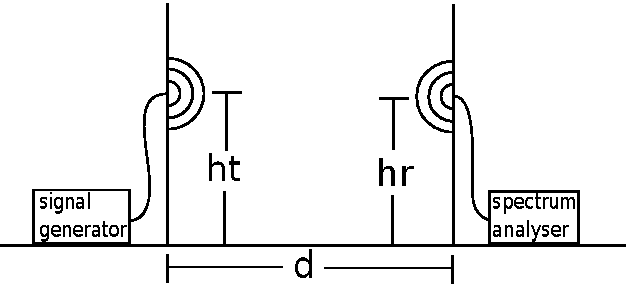
\includegraphics[width = 0.8\columnwidth]{figures/setup.pdf}
\end{figure}
\begin{minipage}{0.15\textwidth}
 \textcolor{white}{.}  
\end{minipage}%
\begin{minipage}{0.8\textwidth}
\begin{itemize}
\item Polarisering
\begin{itemize}
\item Lodret og vandret polarisering
\end{itemize}
\item Lokationer
\begin{itemize}
\item Vind og vejr for udendørs
\item Vægge og pladskapacitet for indedørs
\item Tilgængelighed
\end{itemize}
\end{itemize}
\end{minipage}
\end{frame}

\begin{frame}{Parameter bestemmelse}
\begin{figure}[!htbp]
	\centering
	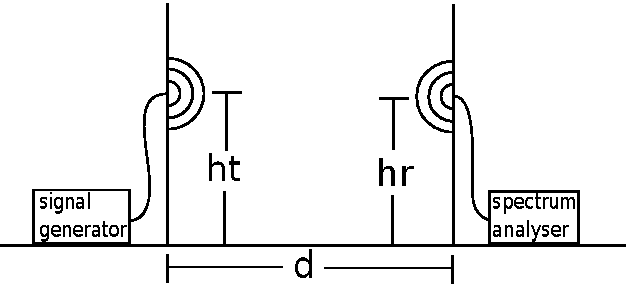
\includegraphics[width = 0.8\columnwidth]{figures/setup.pdf}
\end{figure}
\begin{minipage}{0.15\textwidth}
 \textcolor{white}{.}  
\end{minipage}%
\begin{minipage}{0.8\textwidth}
\begin{itemize}
\item Højder
\begin{itemize}
\item Spejlvending i sender og modtager højderne
\item Flere højder i de lave højder
\end{itemize}
\item Afstande
\begin{itemize}
\item Plads i længde og bredde
\item Logaritmisk fordelt
\end{itemize}
\end{itemize}
\end{minipage}
\end{frame}


\begin{frame}{Parameter bestemmelse}
\begin{figure}[!htbp]
	\centering
	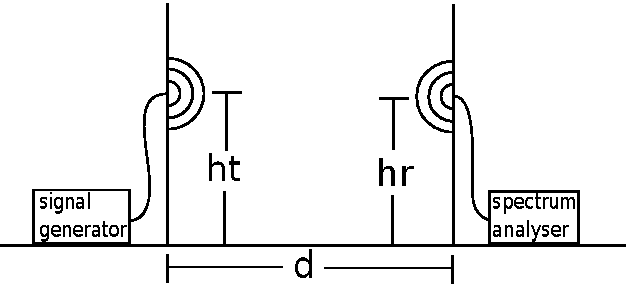
\includegraphics[width = 0.8\columnwidth]{figures/setup.pdf}
\end{figure}
\begin{minipage}{0.15\textwidth}
 \textcolor{white}{.}  
\end{minipage}%
\begin{minipage}{0.8\textwidth}
\begin{itemize}
\item 1 Frekvenser (858 MHz)
\item 2 Antenne par (monopol and patch)
\item 2 Polarisering (vandret and lodret)
\item 2 Lokationer (inde- og udendørs)
\item 10 Rx/Tx højder kombinationer (fra 0.04 til 2.02 m)
\item 6 Afstande (fra 1 til 30 m)
\item Total : 4800 målinger
\end{itemize}
\end{minipage}
\end{frame}